\documentclass[a4paper]{article}
%\usepackage[T1]{fontenc}
\usepackage[english]{babel}

\usepackage{amsmath}
\usepackage{amssymb,amsfonts,textcomp, graphicx}
\usepackage{graphics}

\usepackage{wrapfig}

\usepackage{parskip}

\usepackage{color}
\usepackage{array}
\usepackage{hhline}
\usepackage{subcaption}

\usepackage{textcomp}

\usepackage[hidelinks]{hyperref}

\setlength\tabcolsep{1mm}
\renewcommand\arraystretch{1.3}

\setlength\voffset{-1in}
\setlength\hoffset{-1in}
\setlength\topmargin{0.7874in}
\setlength\oddsidemargin{0.7874in}
\setlength\textheight{10.118099in}
\setlength\textwidth{6.6932993in}
\setlength\footskip{0.0cm}
\setlength\headheight{0cm}
\setlength\headsep{0cm}

% Code specific

\usepackage{listings}

\definecolor{mygreen}{rgb}{0,0.6,0}
\definecolor{mygray}{rgb}{0.5,0.5,0.5}
\definecolor{mymauve}{rgb}{0.58,0,0.82}

\lstset{ %
  backgroundcolor=\color{white},   % choose the background color; you must add \usepackage{color} or \usepackage{xcolor}
  basicstyle=\footnotesize,        % the size of the fonts that are used for the code
  breakatwhitespace=false,         % sets if automatic breaks should only happen at whitespace
  breaklines=true,                 % sets automatic line breaking
  captionpos=b,                    % sets the caption-position to bottom
  commentstyle=\color{mygreen},    % comment style
  deletekeywords={...},            % if you want to delete keywords from the given language
  escapeinside={\%*}{*)},          % if you want to add LaTeX within your code
  extendedchars=true,              % lets you use non-ASCII characters; for 8-bits encodings only, does not work with UTF-8
  frame=single,	                   % adds a frame around the code
  keepspaces=true,                 % keeps spaces in text, useful for keeping indentation of code (possibly needs columns=flexible)
  keywordstyle=\color{blue},       % keyword style
  language=Octave,                 % the language of the code
  otherkeywords={*,...},           % if you want to add more keywords to the set
  numbers=left,                    % where to put the line-numbers; possible values are (none, left, right)
  numbersep=5pt,                   % how far the line-numbers are from the code
  numberstyle=\tiny\color{mygray}, % the style that is used for the line-numbers
  rulecolor=\color{black},         % if not set, the frame-color may be changed on line-breaks within not-black text (e.g. comments (green here))
  showspaces=false,                % show spaces everywhere adding particular underscores; it overrides 'showstringspaces'
  showstringspaces=false,          % underline spaces within strings only
  showtabs=false,                  % show tabs within strings adding particular underscores
  stepnumber=2,                    % the step between two line-numbers. If it's 1, each line will be numbered
  stringstyle=\color{mymauve},     % string literal style
  tabsize=2,	                   % sets default tabsize to 2 spaces
  title=\lstname                   % show the filename of files included with \lstinputlisting; also try caption instead of title
}

%


\begin{document}

\newcommand\textstyleEmphasis[1]{\textit{#1}}
\renewcommand{\contentsname}{Table des mati\`eres}
\renewcommand\refname{R\'ef\'erences}

\renewcommand{\abstractname}{Pr\'eambule}
\title{\textbf{Projet Conception de Microsyst\`emes \\ Altim\`etre int\'egr\'e en VHDL-AMS}}
\author{Mohamed Hage Hassan \\ Cl\'ement Cheung}
\date{8 Decembre 2017}
\maketitle
\thispagestyle{empty}

\renewcommand{\abstractname}{Pr\'emabule}

\begin{abstract}
La conception des microsyst\`emes micro\'electrom\'ecaniques constitue une comp\'etance importante dans le domaine de la micro\'electronique :
L'int\'egration continue des \'elements de micro-nano dimensions assure la r\'eduction de la taille des circuits mixtes micro\'electronique, qui
peuvent comprendre une multitude de capteurs ainsi que la r\'ealisations des fonctions de plus en plus complexes. \\
Le document pr\'esente les diff\'erentes m\'ethodologies suivies ainsi que les architectures des blocs fonctionels d\'ecrits en VHDL-AMS, ainsi
que l'incorporation et la simulation de mod\`ele de capteur physique et les circuits de traitement. On finalise en effectuant une simulation compl\`ete
du mod\`ele pour caract\'eriser ses performances vis-\`a-vis du cahier des charges.
\end{abstract}

\tableofcontents
\clearpage

\section{Introduction}

\section{Architecture G\'en\'erale de l'altim\`etre}
\section{Mod\'elisation et simulation des blocs}

\subsection{Transducteurs comme \'elements de tests}
\subsection{Capteur de temp\'erature}
\subsection{Architecture de l'amplificateur diff\'erentiel}

\clearpage
\subsection{Convertisseur Analogique-Num\'erique en VHDL-AMS}

\subsubsection{Convertiseur Analogique-Num\'erique 1-bit}

\begin{figure}[!htb]
\begin{center}
  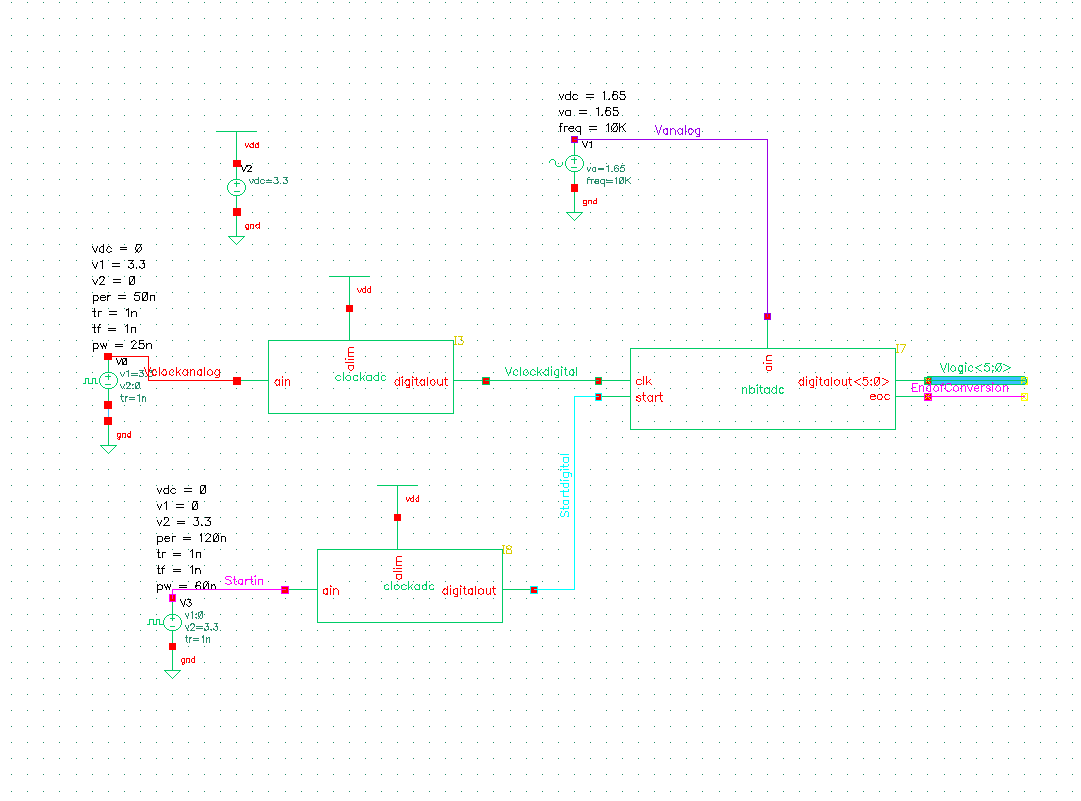
\includegraphics[scale=0.60]{Architecture-ADC-test.png}
  \caption{Sch\'ema g\'en\'eral pour le test de l'ADC 6-bits }
\end{center}
\end{figure}

Utilisation des bibilioth\`eques standards pour les \'el\'ements AMS
\begin{lstlisting}[language=VHDL, belowskip=-0.5 \baselineskip]
library ieee, std;
use ieee.std_logic_1164.all;
use ieee.electrical_systems.all;
\end{lstlisting}

D\'efinitions des terminaux principaux : l'alimentation ainsi que
le signal de la clock est \`a convertir vers une version digitale.
\begin{lstlisting}[language=VHDL, belowskip=-0.5 \baselineskip]
entity clockadc is
	port (
		terminal ain : electrical;  --Analog input terminal
		terminal alim : electrical; --Alim input terminal
		signal Digitalout : out std_ulogic -- Digital 1 bit output
		);
end clockadc;
\end{lstlisting}

\clearpage
L'architecture Conversion\_clock principale de l'ADC, on d\'efinit les
quantit\'es physiques Vin et Vdd pour les tensions d'alimentation et
l'entr\'ee du signal \`a convertir. \textit{lin} et \textit{lalim} seront
d\'efinies \`a 0 pour mod\'eliser l'alimentation et la clock comme sources de tensions
id\'eaux.

\begin{lstlisting}[language=VHDL, belowskip=-0.5 \baselineskip]
architecture Conversion_clock of clockadc is

	quantity Vin across lin through ain to electrical_ref; -- ADC Analog input
	quantity Vdd across lalim through alim to electrical_ref; -- Alim Vdd input

	begin

  -- Process core --

		end process conversion;

	lin == 0.0; -- ideal input
	lalim == 0.0; -- ideal input

end Conversion_clock;
\end{lstlisting}

Le coeur de l'architecture comporte un mod\`ele simplifier pour convertir un signal
analogique d\'epassant une tension de seuil d\'efinie (\textit{Vdd}) vers un bit logique
``1'', ``0'' sinon.
\begin{lstlisting}[language=VHDL, belowskip=-0.5 \baselineskip]
conversion:process(Vin'above(Vdd/2.0))

begin
if Vin'above(Vdd/2.0) then
  Digitalout<= '1';
else
  Digitalout<='0';
end if;
\end{lstlisting}

La simulation d'un tel convertisseur nous remporte des valeurs digitals \`a partir de
celles analogiques.

\begin{figure}[!htb]
\begin{center}
  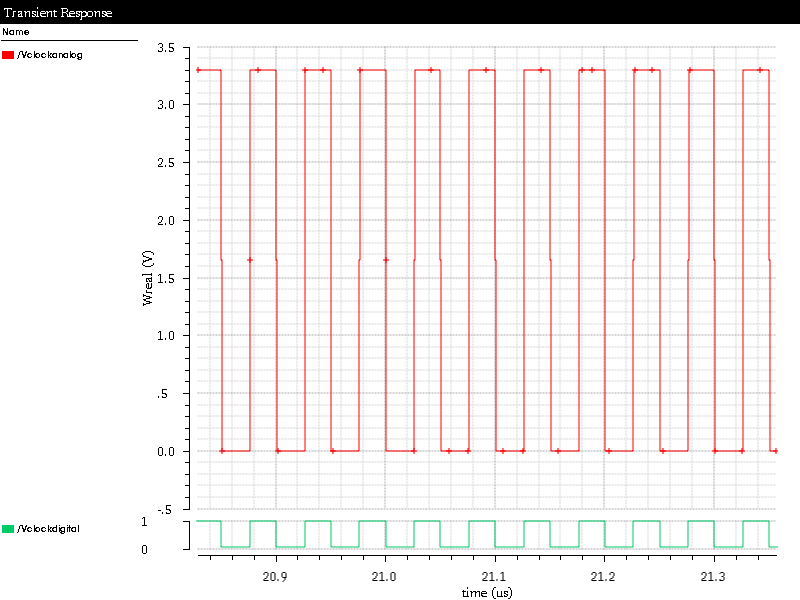
\includegraphics[scale=0.50]{1bit-ADC-conversion-sim.png}
  \caption{Simulation de l'ADC 1-bit }
\end{center}
\end{figure}

\clearpage

\subsubsection{Convertiseur Analogique-Num\'erique 6-bits}

D\'efinition des bibiloth\`eques principaux :
\begin{lstlisting}[language=VHDL, belowskip=-0.5 \baselineskip]
library ieee, std;
use ieee.std_logic_1164.all;
use ieee.electrical_systems.all;
\end{lstlisting}

D\'efinition de l'entit\'e : L'architecture de l'ADC n\'ecessite un signal \textit{start} pour
le d\'eclanchement de l'ADC, une horloge de candancement \textit{clck}, l'entr\'ee
analogique \`a convertire \textit{ain}, le signal de la fin de conversion \textit{eoc}
ainsi qu'un bus en $std\_ulogic\_vector$ qui nous rends les valeurs digitales.
\begin{lstlisting}[language=VHDL, belowskip=-0.5 \baselineskip]
entity nbitadc is
	port (
		signal start: in std_ulogic; -- Start signal from the command logic
		signal clk : in std_ulogic; --clock signal
		terminal ain : electrical;  --Analog input terminal
		signal eoc : out std_ulogic:='0'; -- End of conversion status, initialized on default and used by the command logic
		signal Digitalout : out std_ulogic_vector(5 downto 0) -- Digital 6 bits output
		);
end nbitadc;
\end{lstlisting}

La conversion de l'ADC se d\'eroule dans 2 \'etats diff\'erents \textit{initial, conversion} :
 On d\'ebute par l'intitalisation des valeurs de l'ADS,
\begin{lstlisting}[language=VHDL, belowskip=-0.5 \baselineskip]
architecture Conversion_alpha of nbitadc is
	constant delay:time:=1 ns; -- Conversion time, might be unnecessary
	type adcstates is (initial, conversion); -- Conversion status both initial and on time
	constant bit_range:integer:=5; -- bit range for Digitalout
	quantity Vin across lin through ain to electrical_ref; -- ADC Analog input
	constant Vmax:real:=3.3;

	begin
		convertion_adc:process is
			variable thresh:real:= Vmax;  -- Threshold to test the input voltage against
			variable Vtmp:real; -- Temporary storage of Vin
			variable digital_tmp : std_ulogic_vector(bit_range downto 0); -- Temporary digital output data
			variable actual_status: adcstates:=initial; -- Begin the ADC states with the initial state
			variable bit_cnt:integer:=bit_range;

          -- Process core --

      lin == 0.0; -- ideal input
    end Conversion_alpha;
\end{lstlisting}

\begin{lstlisting}[caption={Coeur du process pour le convertisseur},captionpos=b,language=VHDL, belowskip=-0.5 \baselineskip]
			begin
			case actual_status is

				when initial =>
				wait on start until start='1' or start='H';
					bit_cnt:=bit_range;
					thresh := Vmax;
					Vtmp := Vin;
					eoc<='0';
					actual_status:= conversion; -- Jump to conversion state

				when conversion =>
					wait on clk until clk='1' or clk='H';
					thresh:= thresh/2.0; -- MSB value
					if Vtmp > thresh then
						digital_tmp(bit_cnt):= '1';
						Vtmp := Vtmp - thresh;
					else
						digital_tmp(bit_cnt):='0';
					end if;
					if bit_cnt > 0 then
						bit_cnt := bit_cnt -1;
					else
						Digitalout <= digital_tmp;
						eoc <= '1' after delay; -- End of conversion after a delay
						actual_status := initial;
					end if;
			end case;
		end process convertion_adc;

\end{lstlisting}

\clearpage

\begin{figure}[!htb]
\begin{center}
  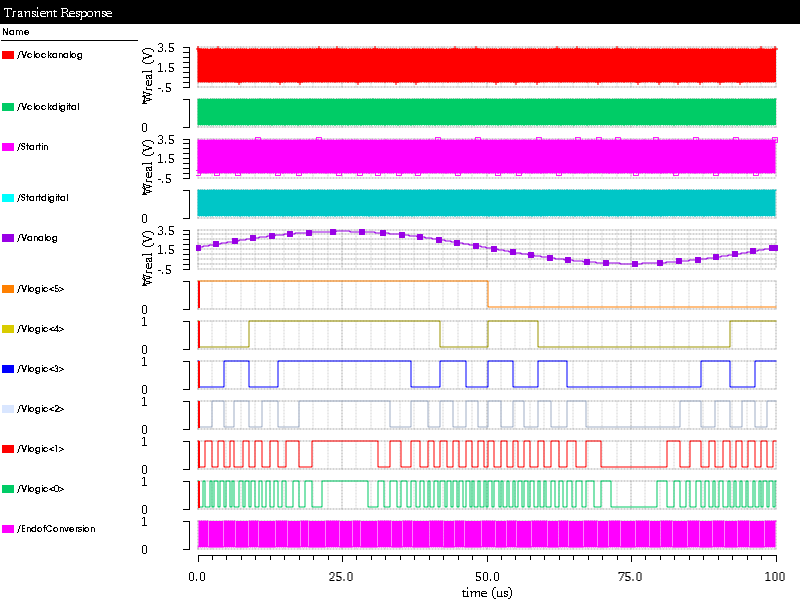
\includegraphics[width=0.7\linewidth]{Simulation-ADC-correct.png}
  \caption{Simulation de totale de l'ADC }
\end{center}
\end{figure}

\begin{figure}[!htb]
\begin{center}
  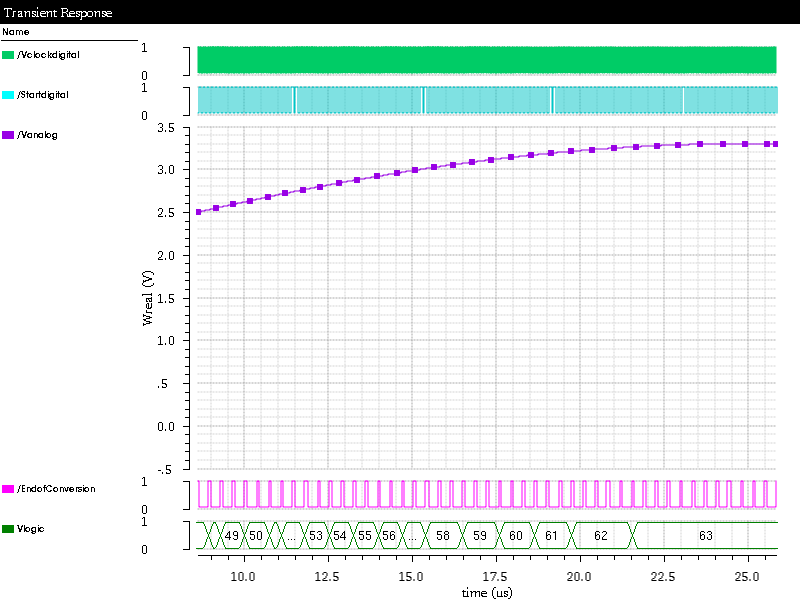
\includegraphics[width=0.7\linewidth]{Simulation-ADC-Bus-correct.png}
  \caption{Simulation de l'ADC}
\end{center}
\end{figure}


\clearpage
\subsection{Logique de commande}


\clearpage

\section{Conclusion}

\clearpage
\section{Annexes}

\subsection{Code complet des blocs VHDL-AMS}

\subsubsection{Convertisseur nbitsADC 6-bits }

\begin{lstlisting}[language=VHDL, belowskip=-0.5 \baselineskip]
library ieee, std;
use ieee.std_logic_1164.all;
use ieee.electrical_systems.all;

entity nbitadc is
	port (
		signal start: in std_ulogic; -- Start signal from the command logic
		signal clk : in std_ulogic; --clock signal
		terminal ain : electrical;  --Analog input terminal
		signal eoc : out std_ulogic:='0'; -- End of conversion status, initialized on default and used by the command logic
		signal Digitalout : out std_ulogic_vector(5 downto 0) -- Digital 6 bits output
		);
end nbitadc;

architecture Conversion_alpha of nbitadc is
	constant delay:time:=1 ns; -- Conversion time, might be unnecessary
	type adcstates is (initial, conversion); -- Conversion status both initial and on time
	constant bit_range:integer:=5; -- bit range for Digitalout
	quantity Vin across lin through ain to electrical_ref; -- ADC Analog input
	constant Vmax:real:=3.3;

	begin
		convertion_adc:process is
			variable thresh:real:= Vmax;  -- Threshold to test the input voltage against
			variable Vtmp:real; -- Temporary storage of Vin
			variable digital_tmp : std_ulogic_vector(bit_range downto 0); -- Temporary digital output data
			variable actual_status: adcstates:=initial; -- Begin the ADC states with the initial state
			variable bit_cnt:integer:=bit_range;

			begin
			case actual_status is

				when initial =>
				wait on start until start='1' or start='H';
					bit_cnt:=bit_range;
					thresh := Vmax;
					Vtmp := Vin;
					eoc<='0';

					actual_status:= conversion; -- Jump to conversion state

				when conversion =>
					wait on clk until clk='1' or clk='H';
					thresh:= thresh/2.0; -- MSB value
					if Vtmp > thresh then
						digital_tmp(bit_cnt):= '1';
						Vtmp := Vtmp - thresh;
					else
						digital_tmp(bit_cnt):='0';
					end if;
					if bit_cnt > 0 then
						bit_cnt := bit_cnt -1;
					else
						Digitalout <= digital_tmp;
						eoc <= '1' after delay; -- End of conversion after a delay
						actual_status := initial;
					end if;
			end case;
		end process convertion_adc;

	lin == 0.0; -- ideal input
	-- lalim == 0.0; --ideal power input

end Conversion_alpha;
\end{lstlisting}


\subsubsection{Convertiseur 1bit clockadc}

\begin{lstlisting}[language=VHDL, belowskip=-0.5 \baselineskip]
library ieee, std;
use ieee.std_logic_1164.all;
use ieee.electrical_systems.all;

entity clockadc is
	port (
		terminal ain : electrical;  --Analog input terminal
		terminal alim : electrical; --Alim input terminal
		signal Digitalout : out std_ulogic -- Digital 1 bit output
		);
end clockadc;

architecture Conversion_clock of clockadc is

	quantity Vin across lin through ain to electrical_ref; -- ADC Analog input
	quantity Vdd across lalim through alim to electrical_ref; -- Alim Vdd input

	begin

			conversion:process(Vin'above(Vdd/2.0))

			begin
			if Vin'above(Vdd/2.0) then
				Digitalout<= '1';
			else
				Digitalout<='0';
			end if;

		end process conversion;

	lin == 0.0; -- ideal input
	lalim == 0.0; -- ideal input

end Conversion_clock;
\end{lstlisting}



\clearpage


\clearpage
\addcontentsline{toc}{section}{R\'ef\'erences}

\begin{thebibliography}{9}

\bibitem{sim-elec-cours}
\textit{The System Designers Guide to VHDL-AMS Analog, Mixed-Signal, and Mixed-Technology Modeling,}\\
\texttt{Peter J. Ashenden, Gregory D. Peterson and Darrell A. Teegarden, Morgan Kaufmann Publishers Inc}

\end{thebibliography}


\end{document}
